\chapter{Theoretical Foundations}
In this chapter, the theoretical Foundations of deep learning model will be introduced. 
\section{Basis of deep neural network}
\subsection{Basic concept}
    In \cite{Goodfellow-et-al-2016}, the concept of deep learning is well described. The deep learning is actually a solution that allows 
    computer to learn from the experiences and understand the world. The entire world consists of hierarchical concepts and relations between 
    each concept with the simpler concept in the next level are also included. This concept of structural hierarchy allows computers to learn 
    from some simple concepts to deeper concepts to solve complex problems, see \autoref{Computer learns from the hierarchical structure of concepts}.
    \begin{figure}
		\centering
		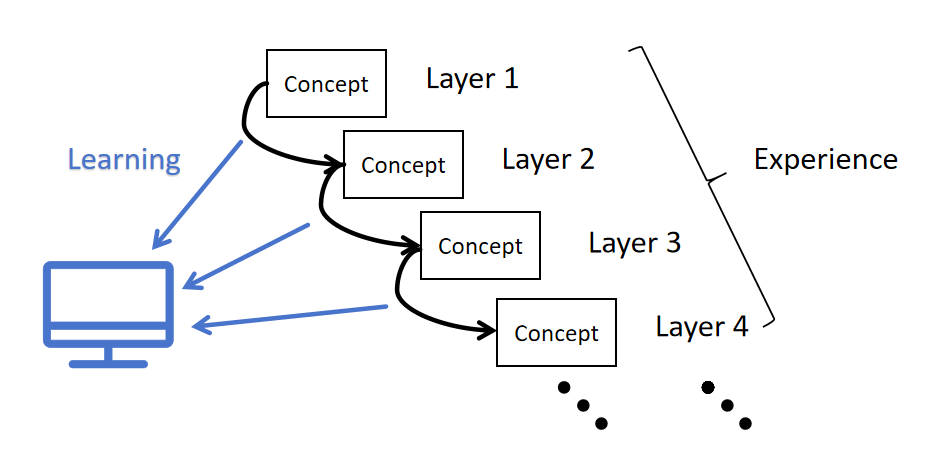
\includegraphics[width=0.6\linewidth]{example_images/ConceptDL}
		\caption{Computer learns from the hierarchical structure of concepts}
		\label{Computer learns from the hierarchical structure of concepts}
	  \end{figure}
    The more layers the structure has, the deeper concepts the computer can learn. After the learning, computers can predict phenomenon and make decisions 
    based on what they have learned. The high-level schematic could be summarized in \autoref{The high-level schematic of deep learning}. The phenomenon or object 
    of interests is the input of the deep learning model. Some simple features will be extracted through sensors, for example the image of the wire harness is extracted 
    through RGB-Camera. The following deep neural network(DNN) can extract more abstract features from the simple features and the computer learns the relations between 
    the features after different layers. After the DNN, the further extracted abstract features should be mapped to the output.  
    \begin{figure}
      \centering
      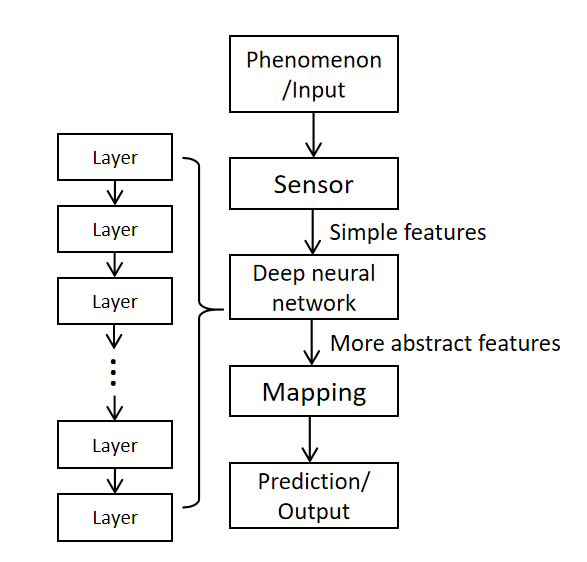
\includegraphics[width=0.6\linewidth]{example_images/DeepLearningSchematic}
      \caption{The high-level schematic of deep learning}
      \label{The high-level schematic of deep learning}
    \end{figure}
  \subsection{Mathematical formulations}
  \subsubsection{Layers}
  The basic principles of how deep learning works were clarified in the previous section. The next questions are: what is the layer? How does it work to extract features?\\
  In order to answer these two questions more intuitively, mathematical expressions should first be defined. The input simple feature should is defined as $x_{0}$. 
  And the next extracted abstract features are defined as $x_{l}$, where l presents the level of the layer, see \autoref{Mathematical explanation of the feature extraction by layers}.
  The layers are actually defined as some first-order linear mathematical expressions $L _{l}$ with the nonlinear activation function $\Phi_{l}$ in \autoref{eq:layer}, 
  where $w$ is the weight and $b$ is the bias. The nonlinear activation function is important. Without it, the output could be just represented from input by one single layer linearly,
  which is not enough to learn the most of the concepts in the world. Some activation functions are explained in \cite{0706bf17a845490688ef4d7d19df65ba}, e.g., ReLU in \autoref{eq:ReLU}, 
  Sigmoid in \autoref{eq:Sigmoid}, Softmax in \autoref{eq:softmax}. The final step of Schematic, Mapping, can actually be regarded as a layer, which has different options depending on 
  the specific task. For example, for classification, the output layer could be softmax, because it maps the features to probabilities. 
  \begin{figure}
    \centering
    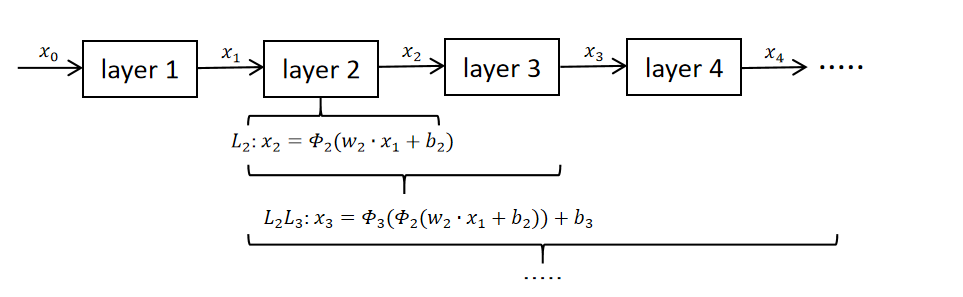
\includegraphics[width=0.9\linewidth]{example_images/mathLayers}
    \caption{Mathematical explanation of the feature extraction by layers}
    \label{Mathematical explanation of the feature extraction by layers}
  \end{figure}
  \begin{align}
    x_{l}=\Phi _{l}(w_{l} \cdot x_{l-1}+ b_{l-1})
     \label{eq:layer}
  \end{align}

  \begin{align}
    \Phi(x) = \begin{cases}
      x& \text{ if } x\ge 0 \\
      0& \text{ else } 
    \end{cases}
     \label{eq:ReLU}
  \end{align}


  \begin{align}
    \Phi(x) = \frac{1}{1+exp(x)^{-1}}  
     \label{eq:Sigmoid}
  \end{align}

  \begin{align}
    \Phi(x_{i}) = \frac{exp(x_{i})}{\sum_{j}exp(x_{j}) } 
     \label{eq:softmax}
  \end{align}
  \subsubsection{Optimization through backpropagated}
  So far, the process of how initial simple features are extracted and transformed step by step into deeper features through different layers and finally mapped into outputs, 
  i.e., predictions, has been well explained. Then a further question follows: how do networks make accurate predictions?\\
  The transformations and mapping are basically performed by \autoref{eq:layer}. Its result is determined by the activation function $\Phi$, weights $w$ and bias$b$. 
  A GroundTruth $y^{\star }$ needs to be artificially introduced to guide the network to learn the correct behavior, i.e. to predict the desired output. This is explained as
  learning from examples and is explained in \cite{russel2010}, which is also well-known as supervised learning. \\
  The prediction of the model or the output after mapping is defined as $y$. A Loss function could be derived. y is actually the result of Mapping, which is actually the output 
  of activation function $\Phi(x)$. It can be further backpropagated onto the feutures from last layer. The optimal weight $w^{star}$ and bais $b^{star}$ are obtained by 
  minimizing the loss equation, see \autoref{eq:Optimization by loss function}. 
  \begin{align}
    w_{l-1}^{\star}, b_{l-1}^{\star}=arg\min_{w_{l-1},b_{l-1}}(\Phi_{l}(\Phi_{l-1}(w_{l-1}\cdot x_{l-1}+b_{l-1}))-y^{\star } ) 
     \label{eq:Optimization by loss function}
  \end{align}
  This approach of optimization can be backwards until the weights and bias of all Layers in the network have been optimized and updated. The whole process is illustrated in 
  \autoref{Parameters are optimized by backpropagation}.
  \begin{figure}
    \centering
    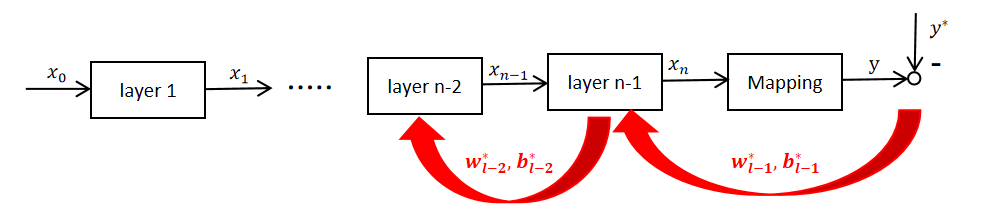
\includegraphics[width=0.9\linewidth]{example_images/bachpropagation}
    \caption{Parameters are optimized by backpropagation}
    \label{Parameters are optimized by backpropagation}
  \end{figure}
  